\documentclass{beamer}
\mode<presentation> {
    \usetheme{Malmoe}
    \usecolortheme{whale}
    \setbeamertemplate{footline}[page number]
    \setbeamertemplate{navigation symbols}{}
}

\usepackage{graphicx} 	% Allows including images
\usepackage{booktabs} 	% Allows the use of \toprule, \midrule and \bottomrule in tables
\usepackage{tikz} 		% Pretty diagrams.
\usetikzlibrary{
    positioning				% Allows 5px above/below of x style positioning
    , arrows				% Allows <-, ->, <-> style arrows.
    , fit					% Allows fitting lines to shapes
    , decorations.pathreplacing	% Allows decoration that affect line paths.
    , shapes.multipart
}

%----------------------------------------------------------------------------------------
%	TITLE PAGE
%----------------------------------------------------------------------------------------

\title[Short title]{NUClear in the NUBots code}

\author{
    Trent Houliston \and Jake Woods
}

\institute[UoN]
{
    University of Newcastle \\ % Your institution for the title page
    \medskip
    \textit{Trent.Houliston@uon.edu.au, Jake.f.woods@gmail.com} % Email address
}

\date{\today}

% Start of document
\begin{document}

%----------------------------------------------------------------------------------------
% Title Slide 
%----------------------------------------------------------------------------------------
\begin{frame}
    \titlepage % Print the title page as the first slide
\end{frame}


%----------------------------------------------------------------------------------------
% Overview (Table of Contents
%----------------------------------------------------------------------------------------
\begin{frame}
    \frametitle{Overview}
    \tableofcontents
\end{frame}

%----------------------------------------------------------------------------------------
\section{Current System}
%----------------------------------------------------------------------------------------
\subsection{Existing Components}
\begin{frame}
    \frametitle{Existing Modules}
	Blackboard
	Jobs
	Hardware Input (CM730)
	Actionators
	Camera
	Vision
	Localization
	Behaviour
	Kinematics
	Team Network
	Game Controller Network
	Configuration System
	Motion
		Scripts
		Head Motion
		Walk Engine
	
\end{frame}

\subsection{Existing Architecture}
\begin{frame}
    \frametitle{Existing Architecture}
    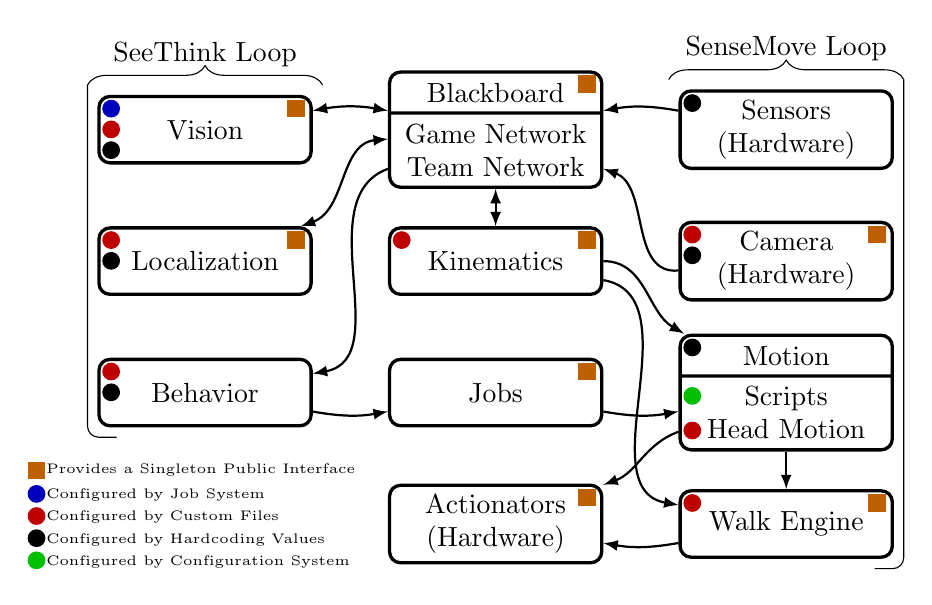
\begin{tikzpicture}[
            x=10.5em,y=4.75em,
            component/.style={
                rectangle
				, rounded corners
                , draw=black, very thick
                , text width=7em
                , minimum height=2.4em
                , text centered
            }
			, splitcomponent/.style={
				component
				, rectangle split
				, rectangle split parts=2
			}
			, configsystemconfig/.style={ color=green!75!black }
			, fileconfig/.style={ color=red!75!black }
			, jobconfig/.style={ color=blue!75!black }
			, hardcodedconfig/.style={ color=black }
			, publicinterface/.style={ color=orange!75!black}
            , write/.style={ ->, thick}
            , read/.style={<-, thick}
            , readwrite/.style={<->, thick}
            , >=latex
        ]

        %\node at (0.5,2.5) {$P_{1}$};

        %%% Nodes
        %% Left hand Side
        \node at (0,3) [component] (vision) {Vision};
        \node at (0,2) [component] (localization) {Localization};
        \node at (0,1) [component] (behavior) {Behavior};

        %% Center
        \node at (1, 3) [splitcomponent] (blackboard) {Blackboard \nodepart{two} Game Network\\Team Network};
		\node at (1, 2) [component] (kinematics) {Kinematics};
		\node at (1, 1) [component] (jobs) {Jobs};
		\node at (1, 0) [component] (actionators) {Actionators (Hardware)};

        %% Right hand side
        \node at(2,3) [component] (sensors) {Sensors (Hardware)};
        \node at(2,2) [component] (camera) {Camera (Hardware)};
        \node at(2,1) [splitcomponent] (motion) {Motion \nodepart{two} Scripts\\Head Motion};
        \node at(2,0) [component] (walkengine) {Walk Engine};

        %%% Connections
        %% Left side connections
        \path [readwrite, out=10, in=170] (vision) edge (blackboard);
        \path [readwrite, out=20, in=185] (localization) edge (blackboard);
        \path [read, out=10, in=200] (behavior) edge (blackboard);
		\path [write, out=-10, in=190] (behavior) edge (jobs);
		
		%% Center connections
        \path [readwrite] (kinematics) edge (blackboard);

        %% Right side connections
        \path [write, out=170, in=10] (sensors) edge (blackboard);
		\path [write, out=185, in=-20] (camera) edge (blackboard);
		\path [write, out=-10, in=190] (jobs) edge (motion);
		\path [write] (motion) edge (walkengine);
		\path [write, out=200, in=20] (motion) edge (actionators);
		\path [write, out=190, in=-10] (walkengine) edge (actionators);
		\path [read, out=150, in=0] (motion) edge (kinematics);
		\path [read, out=170, in=-10] (walkengine) edge (kinematics);
		
		%%% Configuration Colours
		%% Vision
		\filldraw[jobconfig] ([yshift=-.5em,xshift=.5em]vision.north west) circle(3pt);
		\filldraw[fileconfig] ([yshift=-1.25em,xshift=.5em]vision.north west) circle (3pt);
		\filldraw[hardcodedconfig] ([yshift=-2em,xshift=.5em]vision.north west) circle(3pt);
		\filldraw[publicinterface] ([yshift=-.8em,xshift=-0.9em]vision.north east) rectangle ++(6pt, 6pt);	
		
		%% Localization
		\filldraw[fileconfig] ([yshift=-.5em,xshift=.5em]localization.north west) circle(3pt);
		\filldraw[hardcodedconfig] ([yshift=-1.25em,xshift=.5em]localization.north west) circle (3pt);
		\filldraw[publicinterface] ([yshift=-.8em,xshift=-0.9em]localization.north east) rectangle ++(6pt, 6pt);
		
		%% Behavior
		\filldraw[fileconfig] ([yshift=-.5em,xshift=.5em]behavior.north west) circle(3pt);
		\filldraw[hardcodedconfig] ([yshift=-1.25em,xshift=.5em]behavior.north west) circle(3pt);
		
		%% Blackboard
		\filldraw[publicinterface] ([yshift=-.8em,xshift=-0.9em]blackboard.north east) rectangle ++(6pt, 6pt);
		
		%% Kinematics
		\filldraw[fileconfig] ([yshift=-.5em,xshift=.5em]kinematics.north west) circle(3pt);
		\filldraw[publicinterface] ([yshift=-.8em,xshift=-0.9em]kinematics.north east) rectangle ++(6pt, 6pt);
		
		%% Jobs
		\filldraw[publicinterface] ([yshift=-.8em,xshift=-0.9em]jobs.north east) rectangle ++(6pt, 6pt);
		
		%% Actionators
		\filldraw[publicinterface] ([yshift=-.8em,xshift=-0.9em]actionators.north east) rectangle ++(6pt, 6pt);
		
		%% Sensors
		\filldraw[hardcodedconfig] ([yshift=-.5em,xshift=.5em]sensors.north west) circle(3pt);
		
		%% Camera
		\filldraw[fileconfig] ([yshift=-.5em,xshift=.5em]camera.north west) circle(3pt);
		\filldraw[hardcodedconfig] ([yshift=-1.25em,xshift=.5em]camera.north west) circle (3pt);
		\filldraw[publicinterface] ([yshift=-.8em,xshift=-0.9em]camera.north east) rectangle ++(6pt, 6pt);
		
		%% Motion
		\filldraw[hardcodedconfig] ([yshift=-.5em,xshift=.5em]motion.north west) circle (3pt);
		\filldraw[configsystemconfig] ([yshift=-2.25em,xshift=.5em]motion.north west) circle (3pt);
		\filldraw[fileconfig] ([yshift=-3.5em,xshift=.5em]motion.north west) circle(3pt);
		
		%% Walk Engine
		\filldraw[fileconfig] ([yshift=-.5em,xshift=.5em]walkengine.north west) circle(3pt);
		\filldraw[publicinterface] ([yshift=-.8em,xshift=-0.9em]walkengine.north east) rectangle ++(6pt, 6pt);
		
		%%% Legend
		\coordinate (legendpoint) at (.55, .35);
		
		%% Public Interface
		\node [below=3pt of legendpoint,anchor=south east] (publicinterfacelabel) {\tiny Provides a Singleton Public Interface};
		\filldraw[publicinterface] ([yshift=-3pt,xshift=-3pt]publicinterfacelabel.west) rectangle ++(6pt, 6pt);
		
		%% Job Config
		\node [below=0.9em of publicinterfacelabel.south west,anchor=south west] (jobconfiglabel) {\tiny Configured by Job System};
		\filldraw[jobconfig] ([yshift=.5pt]jobconfiglabel.west) circle (3pt);
		
		%% File Config
		\node [below=0.8em of jobconfiglabel.south west,anchor=south west] (fileconfiglabel) {\tiny Configured by Custom Files};
		\filldraw[fileconfig] ([yshift=.5pt]fileconfiglabel.west) circle (3pt);
		
		%% Hard Coded Config
		\node [below=0.8em of fileconfiglabel.south west,anchor=south west] (hardcodedconfiglabel) {\tiny Configured by Hardcoding Values};
		\filldraw[hardcodedconfig] ([yshift=.5pt]hardcodedconfiglabel.west) circle (3pt);
		
		%% Config System Config
		\node [below=0.8em of hardcodedconfiglabel.south west,anchor=south west] (configsystemconfiglabel) {\tiny Configured by Configuration System};
		\filldraw[configsystemconfig] ([yshift=.5pt]configsystemconfiglabel.west) circle (3pt);
		
        %%% Decorations
        %% SeeThink header
        \node[fit=(vision)(localization)(behavior)](leftgroup){};
        \draw[rounded corners] 
        (leftgroup.north west)--(leftgroup.south west) -- ++(0.10,0);            
        \draw[decorate,decoration={amplitude=7pt,brace}] % Header line
        (leftgroup.north west) -- (leftgroup.north east);

        \node[above=1.1em of leftgroup,anchor=center]{SeeThink Loop};

        %% SenseMove header
        \node[fit=(sensors)(camera)(motion)(walkengine)](rightgroup){};
        \draw[rounded corners] 
        (rightgroup.north east) -- (rightgroup.south east) -- ++(-0.10,0);
        \draw[decorate,decoration={amplitude=7pt,brace}]
        (rightgroup.north west) -- (rightgroup.north east);
        \node[above=1.1em of rightgroup,anchor=center]{SenseMove Loop};
    \end{tikzpicture}

\end{frame}

\begin{frame}
    \frametitle{Existing Architecture}
    Description of Existing Architecture
\end{frame}

\subsection{Pain Points}
\begin{frame}
    \frametitle{Pain Points}
	Multiple ways to do the same thing
	Mix of different communication methods
	Threading
\end{frame}

%----------------------------------------------------------------------------------------
\section{NUClear Architecture}
%----------------------------------------------------------------------------------------
\subsection{Architectural Overview}
\begin{frame}
    \frametitle{NUClear Architecure}
	Diagrams
\end{frame}

\begin{frame}
    \frametitle{NUClear Architecure}
	Message passing system,
	Multi Threading,
	Networking,
	Power Plant,
	Reactors,
	Reactions
	Smart Types
	Extensions
	Service Threads
\end{frame}

\subsection{Key Functions}
\begin{frame}
    \frametitle{Key Functions On}
	Trigger
	With
	Code Example
\end{frame}

\begin{frame}
    \frametitle{Key Functions Emit}
	Default
	Scopes
	Unique Pointers
	Code Example
\end{frame}

\begin{frame}
    \frametitle{Key Functions Log}
	Stream operator overload
	variardic
\end{frame}

\begin{frame}
    \frametitle{Antipatterns}
	unending loops in reactions
\end{frame}

%----------------------------------------------------------------------------------------
\section{NUClear in NUBots}
%----------------------------------------------------------------------------------------
\subsection{Module Examples}
\begin{frame}
    \frametitle{Some title}
	Config System
	Party Darwin
	Show examples
\end{frame}

\subsection{Current Porting Status}
\begin{frame}
    \frametitle{Current Porting Status}
	What has been ported
\end{frame}

\end{document} 
